
\chapter{\'Etudes de cas et exp\'erimentations}
\label{experiences.chap}

Ce chapitre pr\'esente une \'evaluation exp\'erimentale de \TT{PpFf} afin d'analyser les possibilit\'es d'utilisation, en termes de performances, par rapport \`a d'autres approches d'ex\'ecution parall\`ele. Chaque exp\'erience est ex\'ecut\'ee plusieurs fois pour obtenir un r\'esultat stable. Dans un environnement de traitement de flux, les donn\'ees sont g\'en\'eralement transform\'ees au fur et \`a mesure de leur progression dans le \TT{pipeline}. Dans les sections suivantes, nous pr\'esentons deux applications de \TT{PpFf}. Ces cas d'utilisation ont \'et\'e choisis non seulement pour montrer certaines fonctionnalit\'es de l'API, mais \'egalement pour leur pertinence dans des sc\'enarios r\'eels. La section~\ref{wordcount.sect} pr\'esente une application permettant de calculer la fr\'equence d'occurrence des mots dans un texte --- le <<\emph{Hello World!} des syst\`emes de traitement de donn\'ees en mode \emph{batch} --- alors que la section~\ref{stockprice.sect} pr\'esente une application permettant de calculer des statistiques sur les prix d'indices boursiers --- un exemple typique de traitement de flux en ligne.


\section{Word Count}
\label{wordcount.sect}

D\'ecrit dans la section.~\ref{descriptionWordCount.sect}, \TT{WordCount} est une application simple qui compte le nombre d'occurrences des divers mots dans un fichier texte. L'application prend en entr\'ee un fichier texte et apr\`es le traitement, sort un conteneur de type \TT{map<string, int>} où la valeur de la cl\'e repr\'esente un mot dans le fichier et la valeur du conteneur de type \TT{int} repr\'esente l'occurrence du mot dans le fichier. Les codes sources des applications \TT{WordCount} dans \TT{PpFf} et \TT{Java} sont list\'es dans l'appendice~\ref{sourceCodeWordCountPpFf.ann} et l'appendice~\ref{sourceCodeWordCountJava.ann} respectivement.



\section{Stock Market}
\label{stockprice.sect}

Dans le monde informatique actuel, les institutions financi\`eres telles que les march\'es boursiers produisent d'\'enormes quantit\'es d'informations. L'un des probl\`emes les plus importants qu'elles rencontrent consiste \`a trouver des moyens efficaces pour r\'esumer et visualiser les donn\'ees boursi\`eres afin de recueillir des informations utiles sur le comportement du march\'e en matière de d\'ecisions d'investissement. Cette section pr\'esente une telle application qui calcule le prix maximum pour chaque stock d'un marché boursier. Les codes sources des applications \TT{StockPrice} dans \TT{PpFf} et \TT{Java} sont list\'es dans l'appendice~\ref{sourceCodeStockPricePpFf.ann} et l'appendice~\ref{sourceCodeStockPriceJava.ann} respectivement. Une telle application est compos\'ee en combinant cinq principales op\'erations.

Les op\'erations d\'efinissant le pipeline sont les suivantes :

\begin{itemize}

\item La premi\`ere op\'eration d'un pipeline sert \`a d\'efinir la source du flux de donn\'ees. Ici, la source est constitu\'ee par les lignes contenues dans un fichier.

\item La deuxi\`eme op\'eration permet de r\'epartir les \'el\'ements du flux entre divers \emph{threads}
Toutes les \'etapes suivant cette op\'eration seront ex\'ecut\'ees en parall\`ele.

\item La troisi\`eme op\'eration, l'op\'eration \TT{map} permet d'extraire le nom et les donn\'ees de chaque stock du march\'e boursier.

\item Le prix pour chaque stock est calcul\'e dans la quatri\`eme op\'eration. L'algorithme utilis\'e est \TT{Black \& Scholes}.

\item La derni\`ere op\'eration du flux permet d'extraire le prix maximum pour chaque stock du march\'e boursier.


\end{itemize}


\section{Mesures}


\subsection{WordCount}

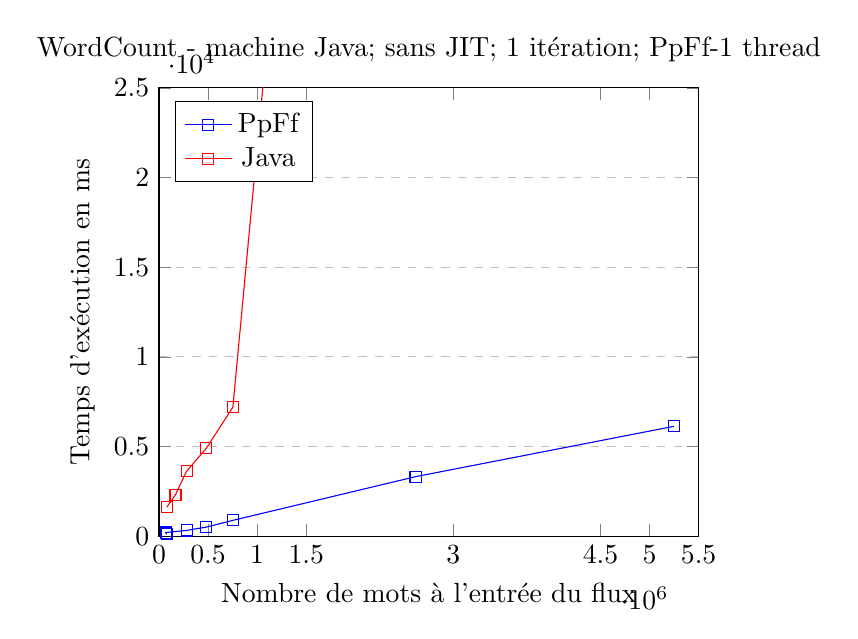
\begin{tikzpicture}
\begin{axis}[
    title={WordCount - machine Java; sans JIT; 1 itération; PpFf-1 thread},
    xlabel={Nombre de mots \`a l'entr\'ee du flux},
    ylabel={Temps d'ex\'ecution en ms},
    xmin=0, xmax=5500000,
    ymin=0, ymax=25000,
    ytick={0,5000,10000,15000,20000,25000},
    xtick={0,500000,1000000,1500000,3000000,4500000,5000000,5500000},
    legend pos=north west,
    ymajorgrids=true,
    grid style=dashed,
]
 
\addplot[
    color=blue,
    mark=square,
    ]
    coordinates {
    (78792,106)(67941,205)(281307,322)(482636,508)(752856,883)(2614743,3320)(5247678,6126)
    };
\addplot[
    color=red,
    mark=square,
    ]
    coordinates {
    (78792,1615)(167941,2319)(281307,3625)(482636,4906)(752856,7195)(2614743,116039)(5247678,226917)
    };
\legend{PpFf,Java}    
\end{axis}
\end{tikzpicture}




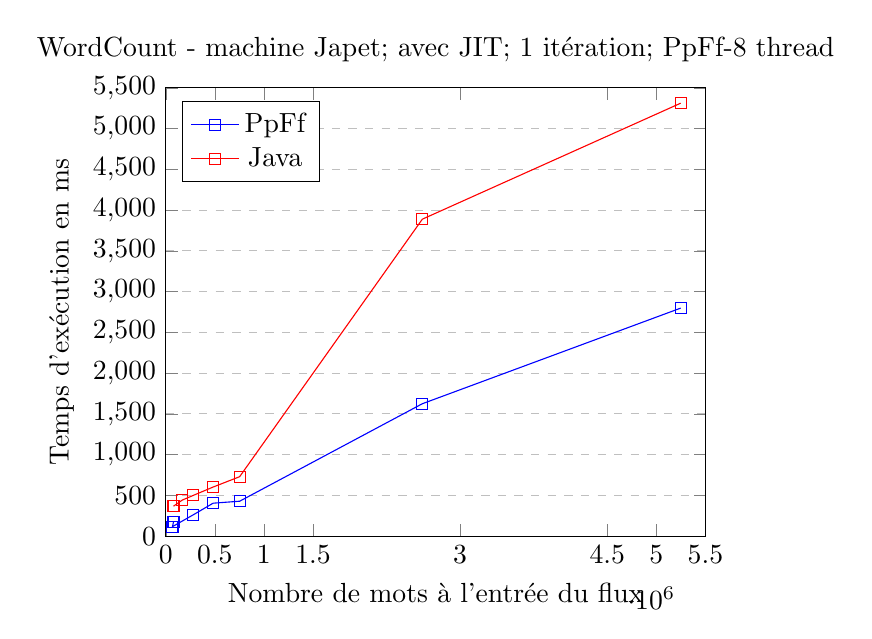
\begin{tikzpicture}
\begin{axis}[
    title={WordCount - machine Japet; avec JIT; 1 itération; PpFf-8 thread},
    xlabel={Nombre de mots \`a l'entr\'ee du flux},
    ylabel={Temps d'ex\'ecution en ms},
    xmin=0, xmax=5500000,
    ymin=0, ymax=5500,
    ytick={0,500,1000,1500,2000,2500,3000,3500,4000,4500,5000,5500},
    xtick={0,500000,1000000,1500000,3000000,4500000,5000000,5500000},
    legend pos=north west,
    ymajorgrids=true,
    grid style=dashed,
]
 
\addplot[
    color=blue,
    mark=square,
    ]
    coordinates {
    (78792,174)(67941,117)(281307,263)(482636,405)(752856,429)(2614743,1625)(5247678,2798)
    };
\addplot[
    color=red,
    mark=square,
    ]
    coordinates {
    (78792,368)(167941,443)(281307,501)(482636,603)(752856,730)(2614743,3889)(5247678,5312)
    };
\legend{PpFf,Java}    
\end{axis}
\end{tikzpicture}








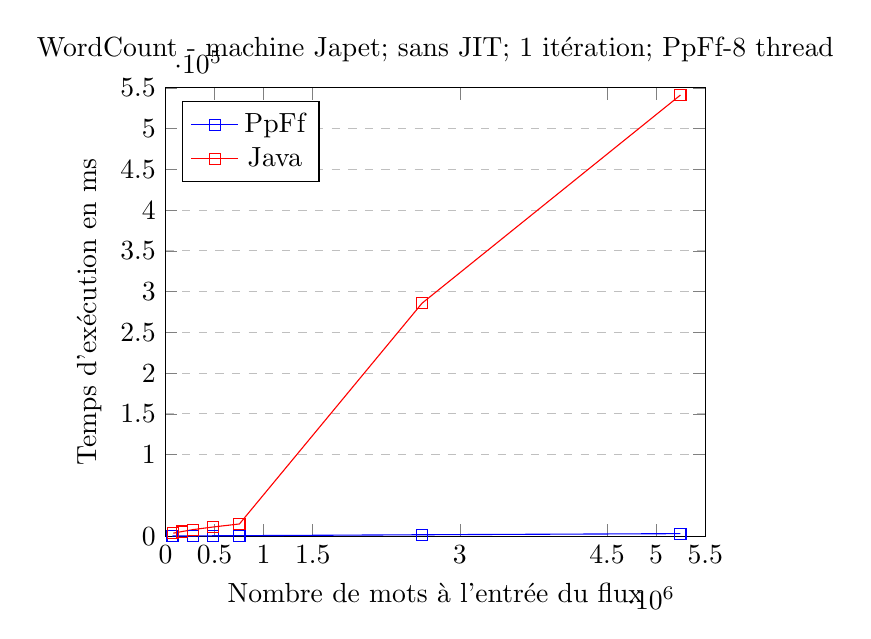
\begin{tikzpicture}
\begin{axis}[
    title={WordCount - machine Japet; sans JIT; 1 itération; PpFf-8 thread},
    xlabel={Nombre de mots \`a l'entr\'ee du flux},
    ylabel={Temps d'ex\'ecution en ms},
    xmin=0, xmax=5500000,
    ymin=0, ymax=550000,
    ytick={0,100000,150000,200000,250000,300000,350000,400000,450000,500000,550000},
    xtick={0,500000,1000000,1500000,3000000,4500000,5000000,5500000},
    legend pos=north west,
    ymajorgrids=true,
    grid style=dashed,
]
 
\addplot[
    color=blue,
    mark=square,
    ]
    coordinates {
    (78792,67)(67941,162)(281307,268)(482636,480)(752856,637)(2614743,1765)(5247678,3135)
    };
\addplot[
    color=red,
    mark=square,
    ]
    coordinates {
    (78792,3685)(167941,5685)(281307,8083)(482636,11258)(752856,14991)(2614743,285866)(5247678,541184)
    };
\legend{PpFf,Java}    
\end{axis}
\end{tikzpicture}


